\documentclass{article}

\usepackage[a4paper]{geometry}

\usepackage[utf8]{inputenc}

% \usepackage{graphics} % Or
\usepackage{graphicx} %% and then \includegraphics[scale=0.5,...]{filename}

%\usepackage[spanish]{babel}
%\usepackage[spanish,english]{babel}

% \usepackage{listings}

% \usepackage{url}
% \usepackage{html}

% \usepackage{fancybox}
% \usepackage{fancyheadings}

% \usepackage{courier}
% \usepackage{times}

\title{Resumen de actividades para reconocimiento de créditos de libre elección}
\author{Adrián Bartol Molina}
\date{30 de Abril de 2010}

\begin{document}
\maketitle

Las actividades a realizar están enmarcadas dentro del proyecto
\emph{Transformers}, un proyecto de transferencia tecnológica de
métodos formales a la industria del ferrocarril. Dentro de dicho
proyecto se estudian varios lenguajes para representar la información
de los requisitos del sistema de ferrocarril europeo (ERTMS).

Entre los diversos lenguajes se encuentran los lenguajes de diagramas
de sequencias (MSC, \emph{Message Sequence Charts}). Las actividades
que me permitirán alcanzar el reconocimiento de los créditos
solicitados son:
\begin{itemize}
\item Diseño de un lenguaje concreto para la representación de MSCs (\emph{Message Sequence Charts}),
\item análisis sintáctico de dicho lenguaje, y
\item análisis de algunas propiedades básicas como la existencia y no duplicidad de identificadores.
\end{itemize}

Este trabajo supone una primera versión de la herramienta
\emph{progtalk} a la que se le añadirán importantes funcionalidades en
mi futuro trabajo de fin de carrera.

Adjunto una planificación bastante detallada de las tareas en las
que se han subdividido las actividades mencionadas anteriormente.

\newpage
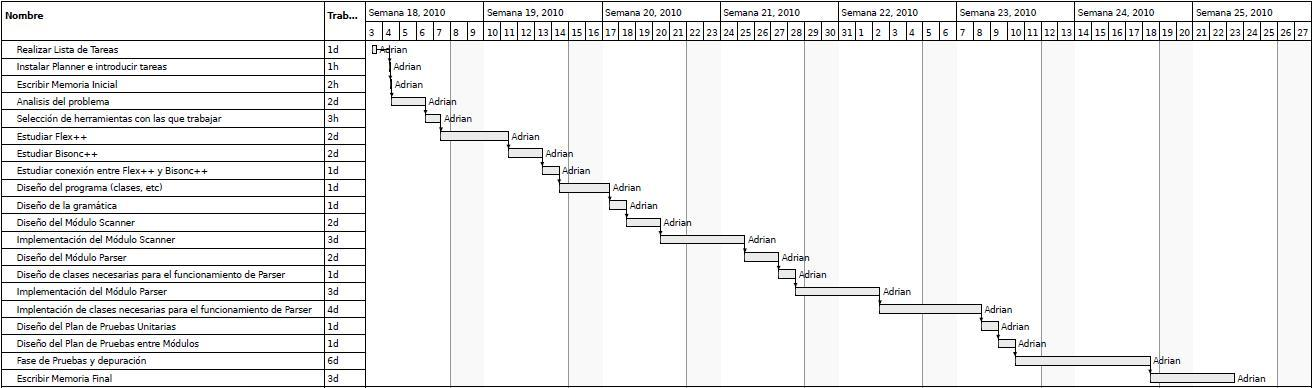
\includegraphics[angle=90,scale=0.7]{planner}
\end{document}

%%% Local Variables: 
%%% mode: latex
%%% TeX-master: t
%%% TeX-PDF-mode: nil
%%% ispell-local-dictionary: "castellano"
%%% End: 

